\section{Natural Language Processing Methodology}
\label{sec:nlp_methodology}

Building on the established causal impact, we now turn to our primary contribution: a comprehensive NLP analysis of how question content, complexity, and focus have evolved in response to ChatGPT's introduction. This section outlines our NLP methodology for detecting and characterizing these changes.

%%%%%%%%%%%%%%%%%%%%%%%%%%%%%%%%%%%%%%%%%%%%%%%%%%%%%%%%%%%%%%%%%%%%%%%%%%%%%%%%%%%%%%%%%%%%%%%%

\subsection{Data Pre-processing}
\textit{[PREPROCESSING PLACEHOLDER - Will detail specific preprocessing steps including tokenization, stopword removal, lemmatization, etc.]}

The resulting word clouds show no immediate clear trend:

\begin{figure}[H]
    \centering
    \begin{subfigure}[b]{0.475\textwidth}
        \centering
        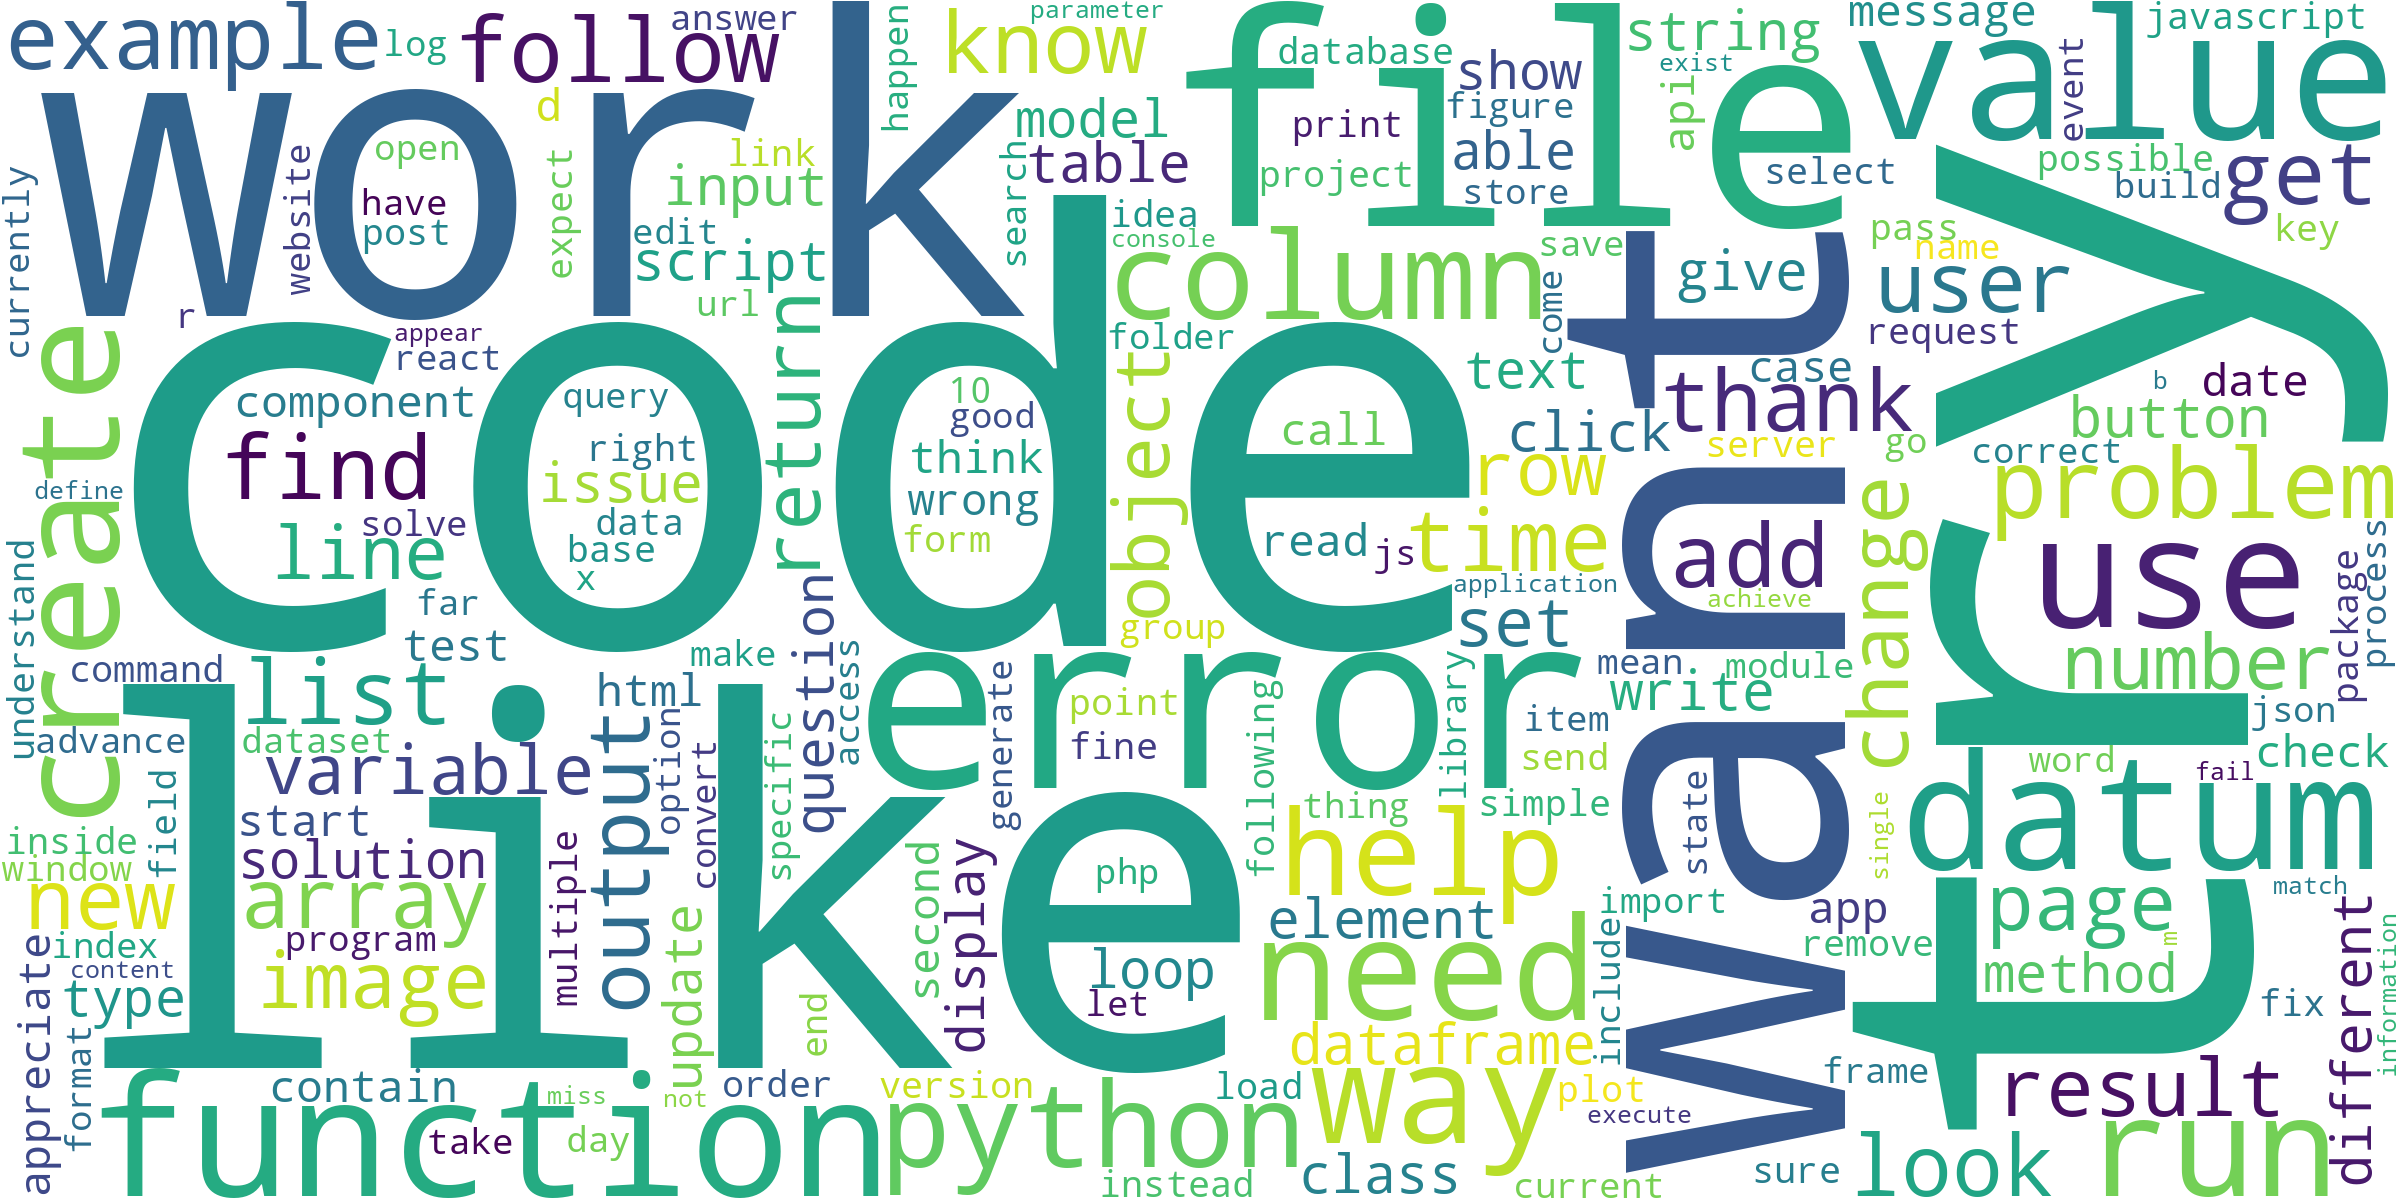
\includegraphics[width=1\linewidth]{imgs/wordclouds/wc_stackoverflow_pre_alphanum.png}
        \caption{Pre-treatment wordcloud}
        \label{fig:prewc}
    \end{subfigure}
    \hfill
    \begin{subfigure}[b]{0.475\textwidth}
        \centering
        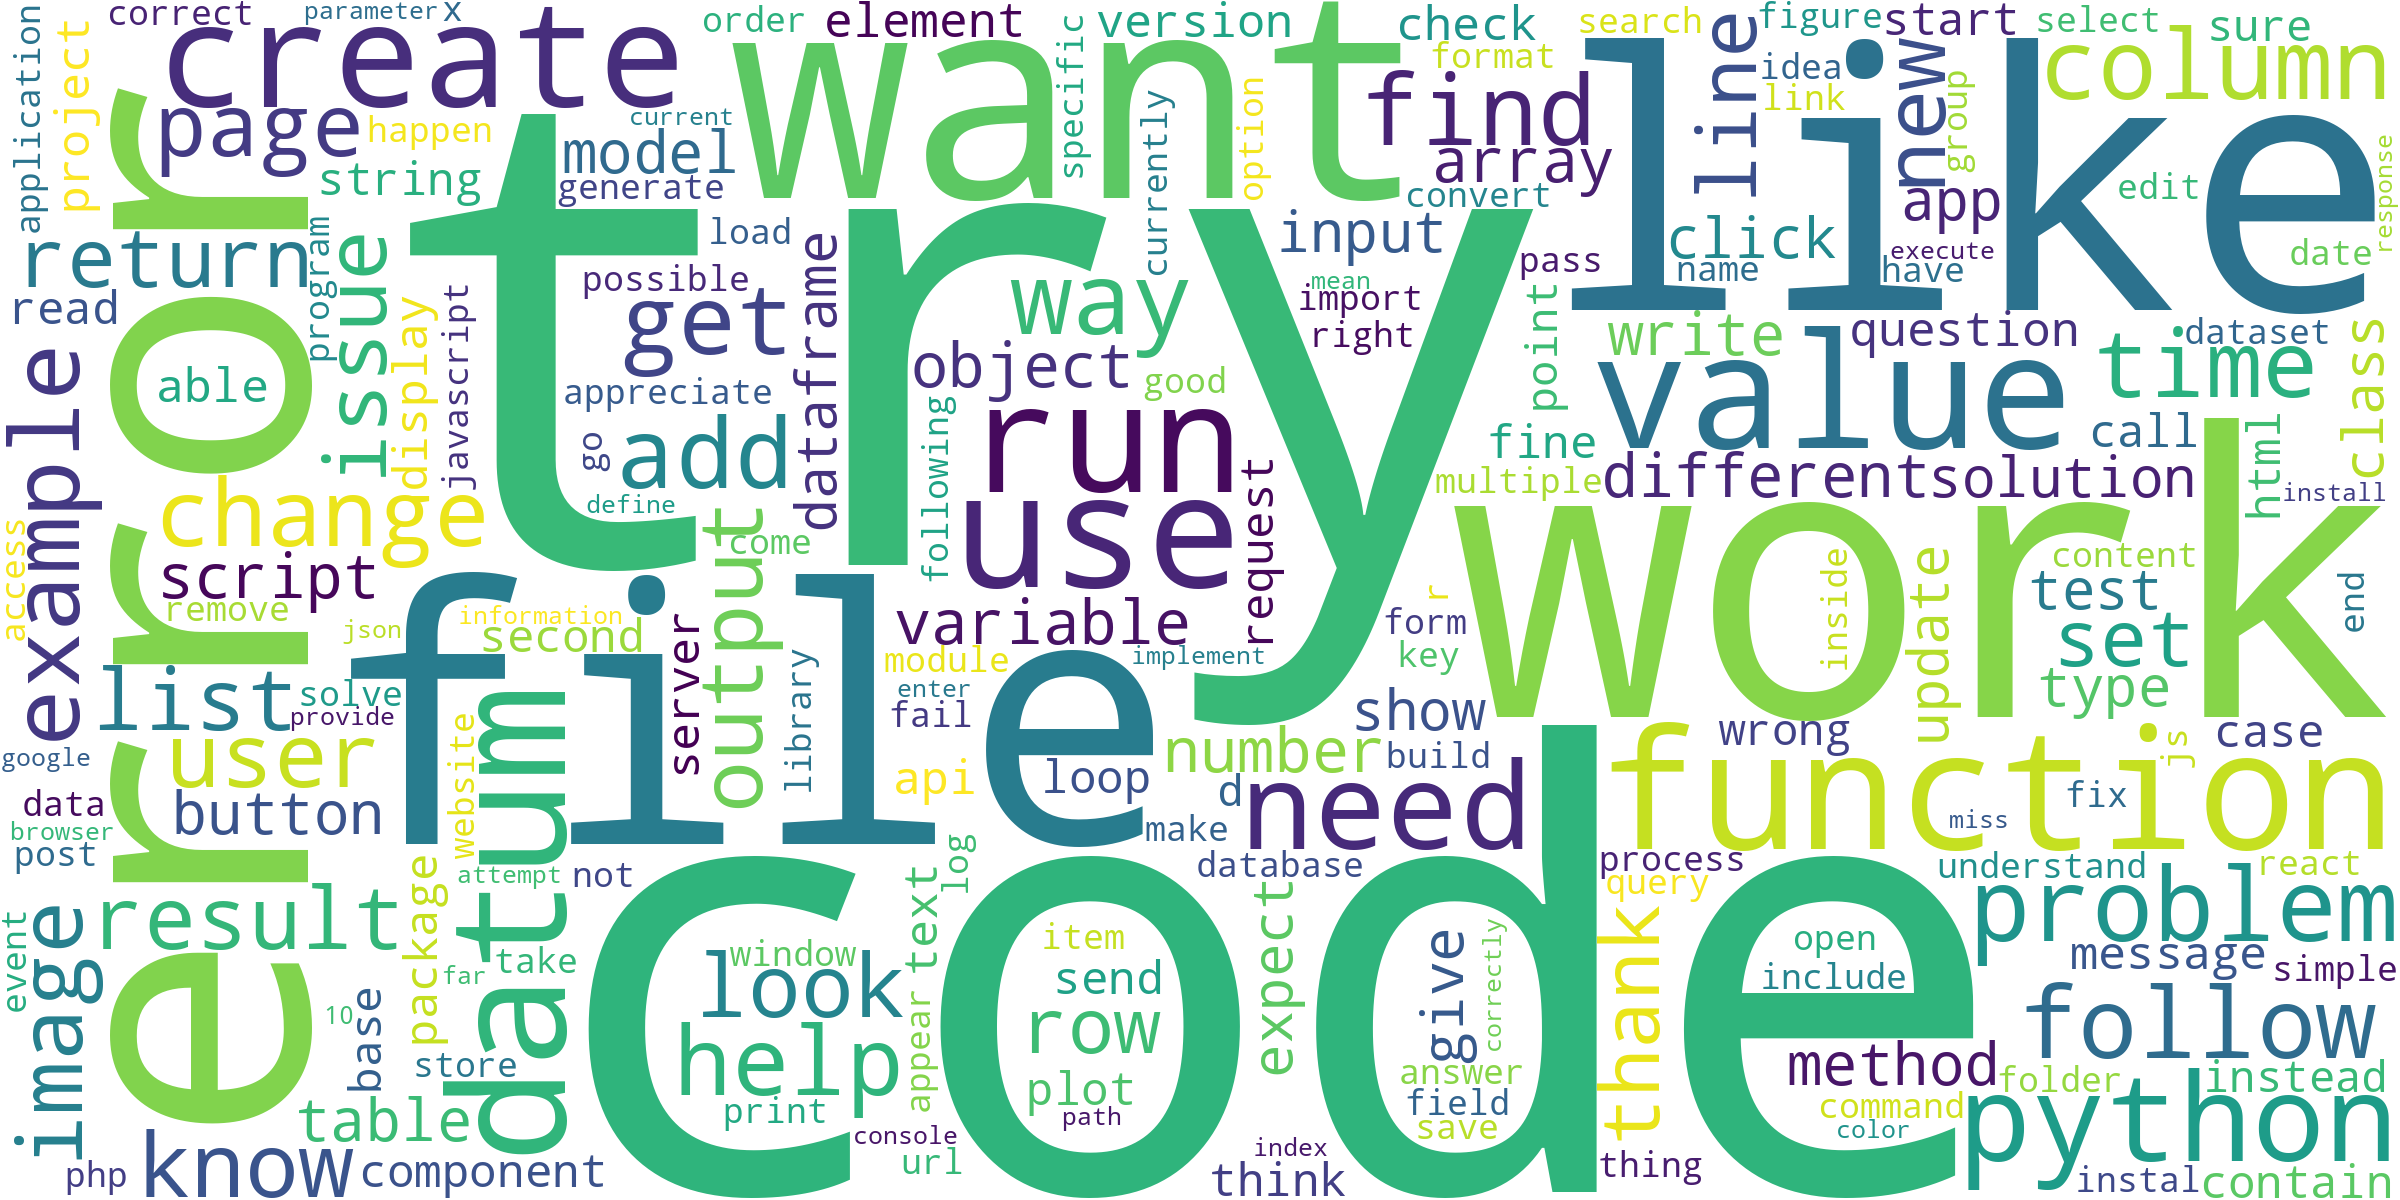
\includegraphics[width=1\linewidth]{imgs/wordclouds/wc_stackoverflow_post_alphanum.png}
        \caption{Post-treatment wordcloud}
        \label{fig:postwc}
    \end{subfigure}
\end{figure}

%%%%%%%%%%%%%%%%%%%%%%%%%%%%%%%%%%%%%%%%%%%%%%%%%%%%%%%%%%%%%%%%%%%%%%%%%%%%%%%%%%%%%%%%%%%%%%%%

\subsection{Topic Modeling}
\textit{[TOPIC MODELING PLACEHOLDER - Will describe topic modeling approach (e.g., LDA), parameter selection, and validation strategies]}

%%%%%%%%%%%%%%%%%%%%%%%%%%%%%%%%%%%%%%%%%%%%%%%%%%%%%%%%%%%%%%%%%%%%%%%%%%%%%%%%%%%%%%%%%%%%%%%%

\subsection{Complexity Analysis}

We construct a parsimonious complexity score for forum posts which is composed of 4 key elements: (1) title length, (2) body length, (3) number of tags and (4) number of code, math, or equation length for the respective forums. The choice of this rather simple score is that questions often just use snippets of code or equations, and thus more sophisticated and established equation or code complexity algorithms become unusable. The results are interesting anyways:


